\documentclass[letterpaper]{article} % Feel free to change this
\usepackage[utf8]{inputenc}
\usepackage{fancyvrb}
\usepackage{listings}
\usepackage{placeins}
\usepackage{amsmath}
\usepackage{graphicx}
\usepackage{rotating}
\begin{document}





\title{ECE 350: Digital Systems Project Checkpoint 4}
\author{Belal Taher} % Change this to your name
\date{March 4th, 2018} % Change this to the date you are submitting
\maketitle

\section*{Duke Community Standard}

By submitting this \LaTeX{} document, I affirm that
\begin{enumerate}
    \item I understand that each \texttt{git} commit I create in this repository is a submission
    \item I affirm that each submission complies with the Duke Community Standard and the guidelines set forth for this assignment
    \item I further acknowledge that any content not included in this commit under the version control system cannot be considered as a part of my submission.
    \item Finally, I understand that a submission is considered submitted when it has been pushed to the server.
\end{enumerate}

\section{Implementation details of previous components}

\subsection{RegFile}

    In order to implement my RegFile, I created 31 32-bit registers in parallel. The reason there are only 31 registers is because register 0 should always contain 0. In order to accomplish this, I hardcoded register 0 to ground. I will talk more about this when I visit how I implemented reading from registers. Each one of my 32-bit registers contains 32 1-bit D flip-flops in parallel. This allows each register to store 32 bits (1 bit in each D flip-flop). \\
    
    Now, I will describe how I implemented writing to a register. All the registers' input ports are connected to data\_writeReg which is the value that should be written to the register represented by ctrl\_writeReg. To implement this, I keep all the registers' write enables turned off besides the one that is represented by ctrl\_writeReg. In order to figure out which register's write enable should be turned on, I use a 5-to-32 decoder. The decoder takes in a 5 bit input and, based on the unsigned representation of that input, sets one of its 32 outputs to VCC and the rest to ground (i.e. 00100 in binary is 4 in decimal so the 4$_{th}$ output port would be set to high while the rest would low). Output one is set to high when the input is 00000 but this output is left dangling. The reason for this is because we should never be able to write to register 0 as it is the zero register and should always contain all zeros. Output two is set to high when the input is 00001 and is hooked up to register 1's write enable. Output three is set to high when the input is 00010 and is hooked up to register 2's write enable e.t.c. This design makes it so that the one register whose write enable is turned on is the register that corresponds to the unsigned represented of ctrl\_writeReg. Having the write enable turned on allows the 32 bit data\_writeReg to be stored in the 32 D flip-flops in the corresponding register. \\
    
    The reason I chose this implementation for writing was because it allows the operation of writing to 1 of 32 different registers to be done as if you were only dealing with one register. When I say that, I mean the fact that the "one-hot" bit from the 5-to-32 decoder is sent to the respective register's write enable in parallel with the 31 other "not-hot" bits and the data\_writeReg is hooked up to all the registers' inputs in parallel allows us to write to one of our registers at the same speed that we would write to only a single register (granted a gate delay from the 5-to-32 decoder). \\
    
    Next, I will describe how I implemented reading from a register. I connected the output of all the 32 registers to two 32-to-1 MUXs: one MUX's output is data\_readA (let's call it MUX A) and the other MUX's output is data\_readB (let's call it MUX B). MUX A's select bits are ctrl\_readA and MUX B's select bits are ctrl\_readB. The reason for this is because ctrl\_readA and ctrl\_readB represent the binary representation of the registers we need to read from (i.e. if ctrl\_readA is 11111 we pass register 32's output value to data\_readA; 11111 corresponds to 32 instead of 31 because 00000 corresponds to register 1). So if the RegFile received 00001 as ctrl\_readA and 00010 as ctrl\_readB, MUX A would know to pass register 2's output to data\_readA and MUX B would know to pass register 3's output to data\_read B. Since register 0 should be always be kept at 0, the output for both MUXs when the select bits of either are 00000 is hardcoded to ground (represented by 32 0's). \\ 
    
    The reason I chose this implementation for reading was because it allows the operation of reading from 2 of 32 different registers very efficiently. When I say that, I mean the fact that all the 32 outputs from our registers are hooked up to two MUXs in parallel allows us to essentially read from the registers of our choice at the same speed that we would read from a single register (granted a gate delay from the 32-to-1 MUX). And, although we have two MUXs, the gate delay is still only that of one MUX since they operate in parallel. \\
    
    I tested this implementation by trying to vary my ctrl\_writeEnable along with my data\_writeEnable to assign unique values to distinct registers (to make sure the values were actually being written to the right registers). Then, I checked to see what outputs came out for data\_readA and data\_readB as I varied my ctrl\_readA and ctrl\_readB bits. \

    
\subsection{ALU}

    In order to implement my ALU, I basically designed it so that all the operations that the ALU is capable of execute in parallel and are fed into a MUX that has the ALU opcode as the select bits. Before I justify this design decision, I'll quickly talk about how I actually implemented all the different operations.
    
    The first operation I implemented was adding. In order to try and maximize efficiency, I created a hierarchical carry-lookahead adder. What makes this adder more efficient is that it uses the idea of a generate and propagate functions to "lookahead" and see if more significant bit positions will require a $C_{in}$. In a normal ripple-carry adder, the addition at bit position 1 is limited by when the addition at bit position 0 is finished, and the addition at bit position 2 is limited by when the addition at bit position 1 is finished and so on. When we adopt the generate and propagate functions, we are able to concurrently calculate higher bit positions since we already know whether or not we will have a $C_{in}$ before the addition at the bit position that causes the $C_{in}$ is completed. My implementation uses a 4 blocks that each do ripple-carry addition on 8-bits. The $C_{out}$ from each of the blocks is left dangling since it is already calculated based on the generate and propagate function of this respective block and passed onto the next one so that the next 8-bits can concurrently (granted after a small delay where the generate and propagate functions are used to calculate the $C_{in}$) be added. A diagram illustrating the general idea of this adder is provided later in the report. \\
    
    The next operation I implemented was subtracting. In 2's complement, subtraction between A and B is the same adding A and (!B + 1). Instead of creating a whole different hierarchical carry-lookahead adder and feeding it !B+1 as its second input instead of B, I decided to only use one hierarchical carry-lookahead adder but have its second input be the output of a MUX that chooses between B and !B + 1. The reason I chose to do this is because creating a different carry-lookahead adder would require much more gates. By MUXing between B and !B+1 I was able to implement subtraction with only one extra piece of hardware (a 32-bit 2-to-1 MUX). Albeit, this way has a slightly longer delay since the MUXing operation takes time, the slightly longer delay was worth it in my eyes to avoid having to essentially double the amount of hardware present in the circuit. The input to my 32-bit 2-to-1 MUX (i.e. the control bit for subtraction) is the least significant bit of my opcode. The reason for this is because the opcode for addition is 00000 and the opcode for subtraction is 00001 (the only difference is the LSB). Although this causes the MUX to choose the !B + 1 input to the adder when operations occur that aren't subtraction but have a 1 as the LSB, it doesn't matter since I also MUX at the end of my ALU to choose the output from the desired operation. I calculated !B + 1 by creating 32 NOT gates that each have 1 bit of B as an input. I implemented the + 1 by feeding the control bit for subtraction into the $C_{in}$ to the adder. This avoided having to create a separate one-bit adder for that + 1 which prevented unnecessary gate delays and unnecessary additional hardware. \\
    
    The next operation I implemented was AND. Essentially, all I did for AND was 32 AND gates that each take in a bit from bit position X from both A and B (i.e. AND gate 1 would be fed A[0] and B[0], AND gate 2 would be fed A[1] and B[1], e.t.c). This design successfully implemented bitwise AND and kept the delay to the minimum value of one gate delay (which was accomplished since all the AND gates operate in parallel).\\
    
    The next operation I implemented was OR. Essentially, all I did for OR was 32 OR gates that each take in a bit from bit position X from both A and B (i.e. OR gate 1 would be fed A[0] and B[0], OR gate 2 would be fed A[1] and B[1], e.t.c). This design successfully implemented bitwise OR and kept the delay to a minimum value of one gate delay (which was accomplished since all the OR gates operate in parallel). \\
    
    The next operation I implemented was a logical left shift (sll). I implemented this by using 5 left shifters in series. The reason I did this was because I recognized that the shift amount is anywhere from 00000 to 11111 and each bit positions represents whether or not you shift by a certain value. Essentially, what I mean by that is having a shift amount of 00011 means that you shift by 1 and then you shift by 2 (since 00011 maps to 0*2$^4$ + 0*2$^3$ + 0*2$^2$ + 1*2$^1$ + 1*2$^0$ in decimal which equals 3). In order to translate this logic into hardware, I created a 16-bit left shifter, 8-bit left shifter, 4-bit left shifter, 2-bit left shifter, and 1-bit left shifter. The number that we want to shift is first fed into the 16-bit left shifter and I MUX between the output of that shifter and itself. Then the output of that MUX is fed into the 8-bit left shifter and then I MUX between the output of that shifter and the output of the previous MUX and so on. The select bit for each MUX is the corresponding bit in the shift amount input (i.e. if our shift amount was 10100 the 16-bit shifter's MUX would have a select bit of 1, the 8-bit shifter's MUX would have a select bit of 0, the 4-bit shifter's MUX would have a select bit of 1 and so on). \\
    
    The next operation I implemented was a arithmetic right shift (sra). I implemented this using the same exact logic as my left shifter (5 right shifters in series). The only difference is that right shifters pad the right side with the most significant bit when shifting and left shifters pad the left side with 0.
    
       \FloatBarrier

  \begin{figure}[!htb]
        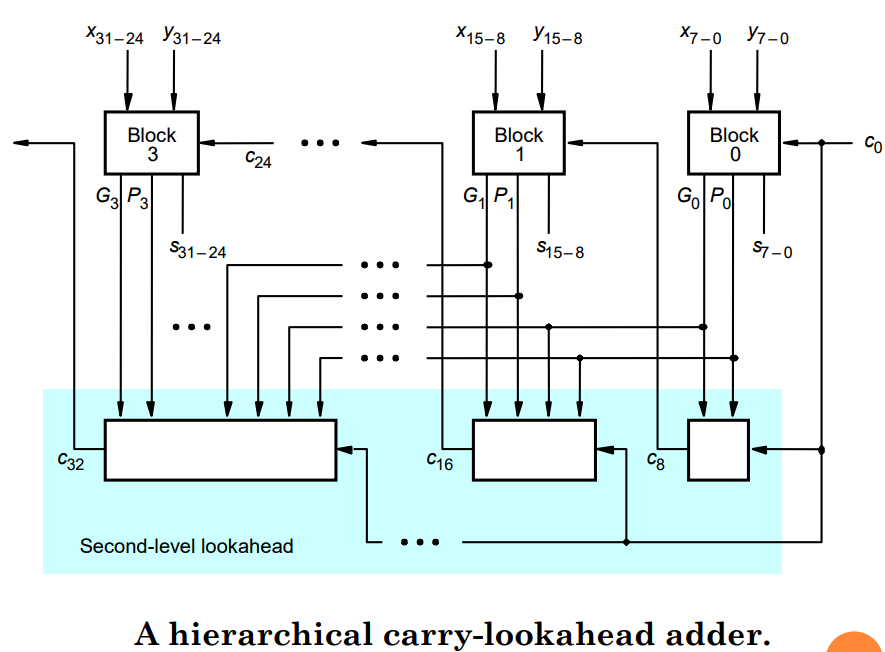
\includegraphics[scale=.5]{HierarchicalCarryLookaheadAdder.PNG}
        \caption{Hierarchical Carry-Lookahead adder schematic}
        \label{fig:2}
    \end{figure}
    
       \FloatBarrier
    
\subsection{MultDiv}

    I did not implement MultDiv for my processor. If I had more time I would have attempted it, but I spent too much time trying to fix hold time violations for all the other operations that I was never able to get around to it. 
    
    
\section{Implementation details of processor design}

\subsection{Fetch}

    My Fetch stage simply has instruction memory, a Program Counter (PC) and a hierarchical carry-lookahead adder. The instruction memory I simply got using the IP catalog that allows you to choose from Quartus' built in components. My Program Counter is a 12 bit register whose output is hooked up to an adder. The adder's other input is a hardcoded one. The reason for this is because the PC increments by 1 word (where words are 32-bits) each time and the convention of the Imem is the input is the word that you currently want to extract. And the reason I use a carry-lookahead adder for a simple addition by 1 is because I wanted to account for the worst cases (i.e. PC = 011111111111 or some other operations that relies heavily on $C_{in}s$) The adder's output is hooked up to a series of MUXs that handle the PC being changed to different values in special cases. I will address these special cases in the instructions section of this report. The output from the series of MUXs is the input to the PC register. This achieves a "counting" effect where the positive clock edge increments the value in the register by 1 each time (assuming none of the special cases trigger). The PC's output is also hooked up to the Imem in which a 32-bit instruction corresponding to the address fed into the Imem is fetched and handed to an 32-bit register (the IR register holds the instruction that was just fetched). A note about my Fetch stage is that the registers are positively clocked and the Imem is negatively clocked. This allows the PC to be incremented in the first half of the clock cycle and the instruction corresponding to the newly incremented PC to be fetched in the second half of the clock cycle. This avoids undefined behavior which would be caused by both the data input and clock changing at the same time. Also, something to note about this design choice is that the instruction at address 0 is always skipped since the Imem doesn't actually fetch an instruction until after the PC register has had its value changed to 1. A diagram of my fetch stage is provided below is better illustrate my Fetch stage.
    
           \FloatBarrier

  \begin{figure}[!htb]
        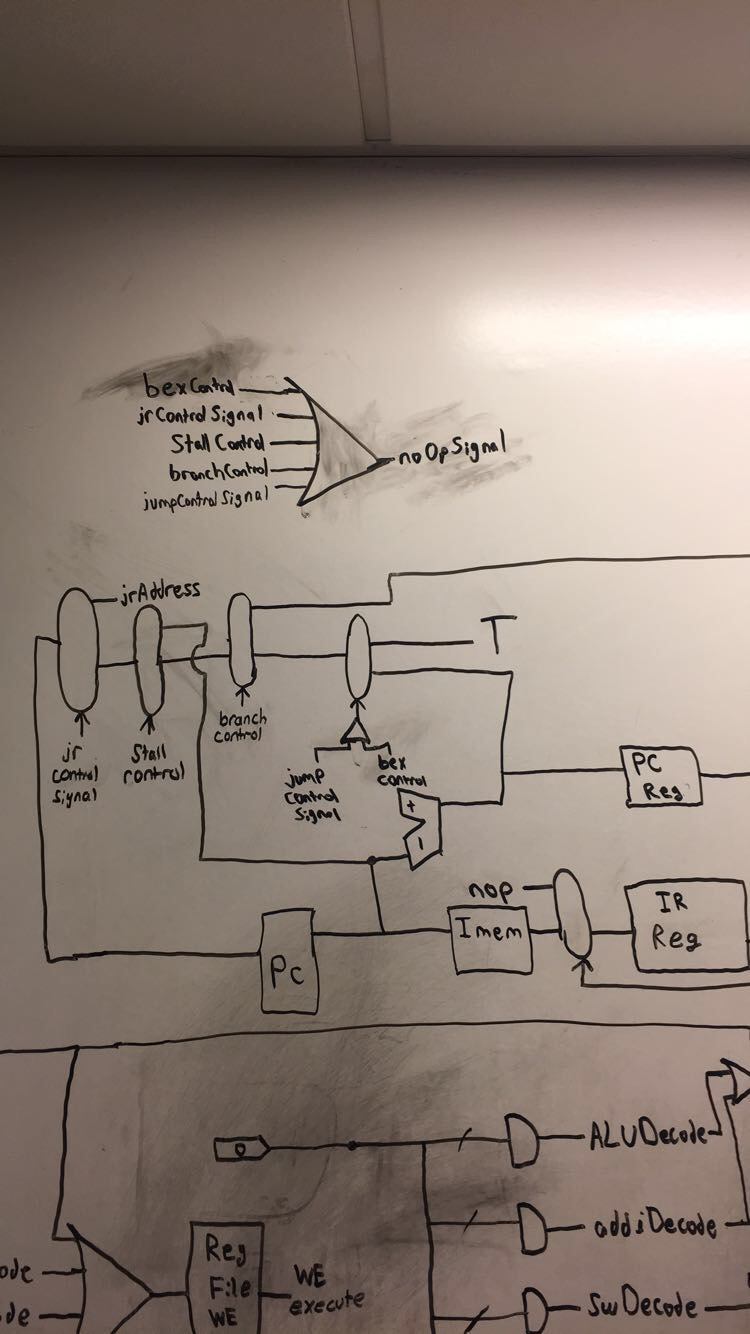
\includegraphics[scale=.45]{Fetch.jpg}
        \caption{Fetch Stage}
        \label{fig:2}
    \end{figure}
    
       \FloatBarrier

\subsection{Decode}

    My Decode stage is where almost all my control signals are calculated. The bits corresponding to various inputs are extracted and stored in registers to be propagated forward in the pipeline (i.e. bits [31:27] are extracted as the opcode and concurrently ran through a series of AND and NOT gates to calculate which instruction is taking place, bits [11:7] are extracted as the shift amount and saved to a register to eventually be fed to the ALU in the next stage, bits [16:0] as the immediate are extracted and saved to a register in case we need the immediate for the command currently executing). The reason I chose to have so many seemingly unnecessary operations occur in the Decode stage (i.e. the reason I extract shift amount when the operation isn't a shift) is because concurrently extracting anything we could ever need is a useful tradeoff in maximizing efficiency. Essentially, instead of having control signals A, B, and C concurrently calculated in Decode and accumulating a gate delay of J and having control signals D and E concurrently calculated in Execute and accumulating another gate delay of K (which in total results in a gate delay of J+K), we have A, B, C, D, and E concurrently calculated in decode and only accumulate a gate delay of max(J,K). We can just MUX the inputs that we actually need in later stages using these control signals.  An example of this is when we do ALU operations vs when we branch (only blt/bne) or jr. ALU operations require \$rs as the A input to the ALU while blt/bne/jr require \$rd as the A input to the ALU. Instead of worrying about which one to extract, we can concurrently extract both and calculate a "rdInA" control signal which is essentially an OR gate between 3 AND gates that output 1 when their corresponding opcode is being decoded (i.e. myjrAnd outputs 1 when the opcode is 00011). Essentially, everything you can extract in the decode stage is extracted and the control signals for later stages are calculated using OR/AND gates based on what's required for them to occur. Some pictures of my decode stage are provided below to give more insight.
    
       \FloatBarrier

  \begin{figure}[!htb]
        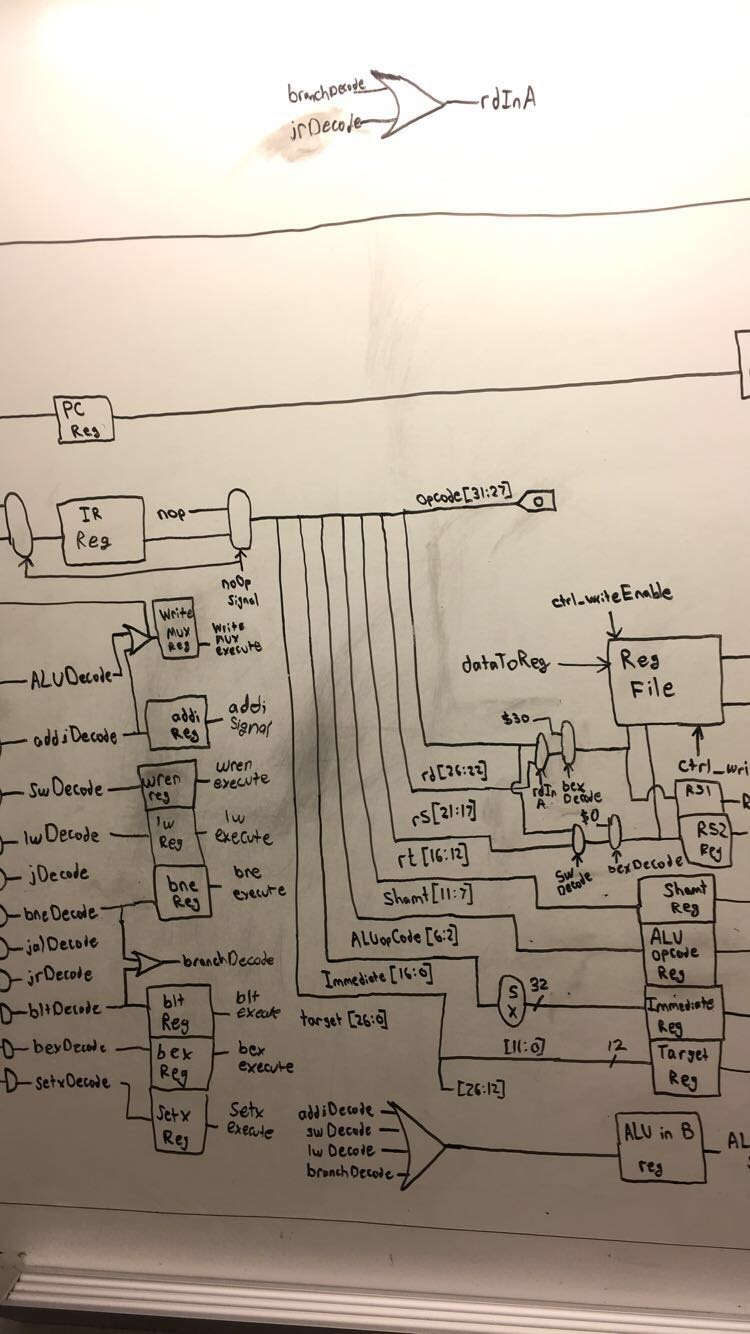
\includegraphics[scale=.4]{Decode1.jpg}
        \label{fig:2}
    \end{figure}


  \begin{figure}[!htb]
        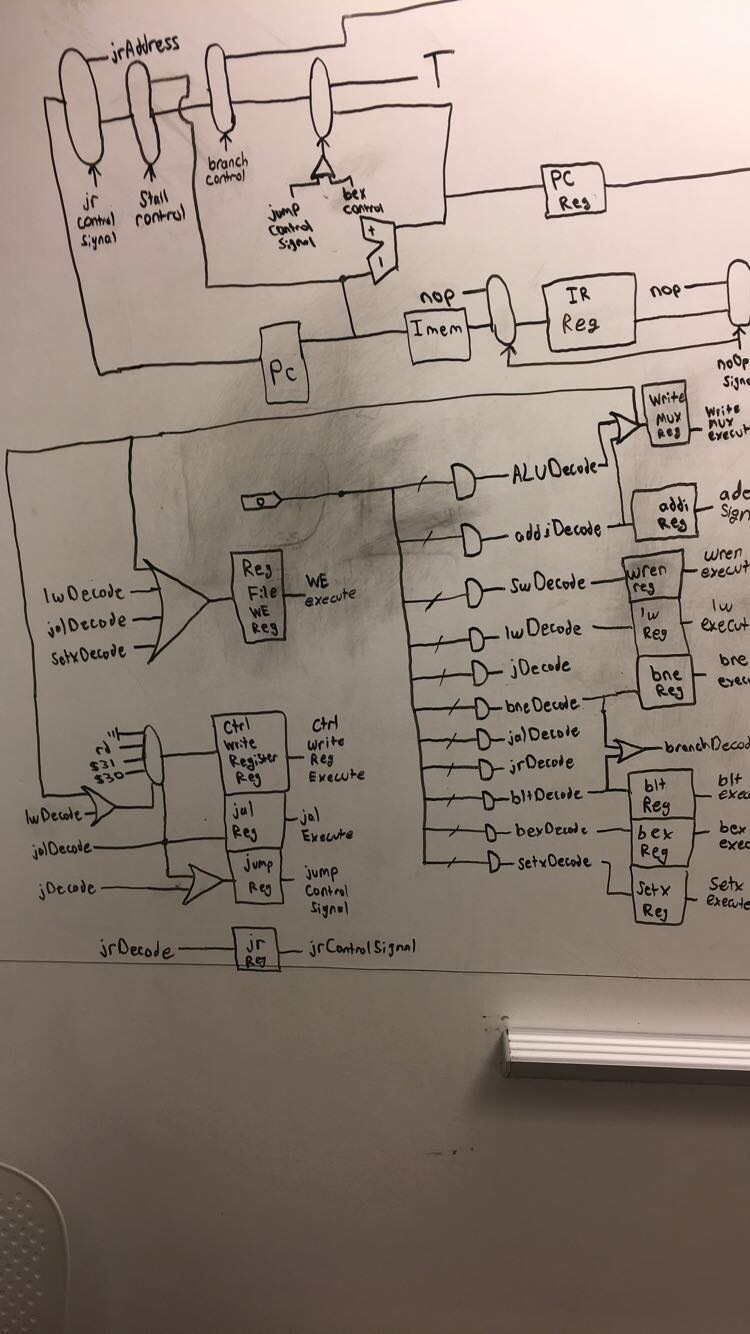
\includegraphics[scale=.4]{Decode2.jpg}
        \caption{Decode Stage}
        \label{fig:2}
    \end{figure}
    
       \FloatBarrier
    
    
    
\subsection{Execute}

    My execute stage doesn't have much going on because of all the work is done in the decode stage. The ALU inputs are chosen by MUXs that operate on control signals that were propagated forward through flip-flops from the Decode stage, and bypass logic is run to see if bypassing is necessary. The ALU is then fed the correct inputs and operates based on the ALU opcode extracted during Decode (propagated forwarded using a 5-bit register). The ALU less than and is not equal outputs are ANDed with the control signals for blt and bne/bex respectively. The convention of my processor is that the Execute stage is where branch conditions and the next PC value (if a command that changes the PC value is being executed) are calculated. The implementation details of the operations the ALU is capable of can be found in section 1.2. My Execute stage also has another adder that constantly adds PC + 1 to the immediate. This is so that whenever a branch occurs, the value to branch to is already computed and can simply be MUXed with what would have been the next PC if the branch didn't occur. A picture of my Execute stage is provided below to better illustrate it. Note that not all the MUXs I ended up using in my final submission are pictured below. The ones that aren't there I will discuss in my instructions' implementation details section.
    
               \FloatBarrier

  \begin{figure}[!htb]
        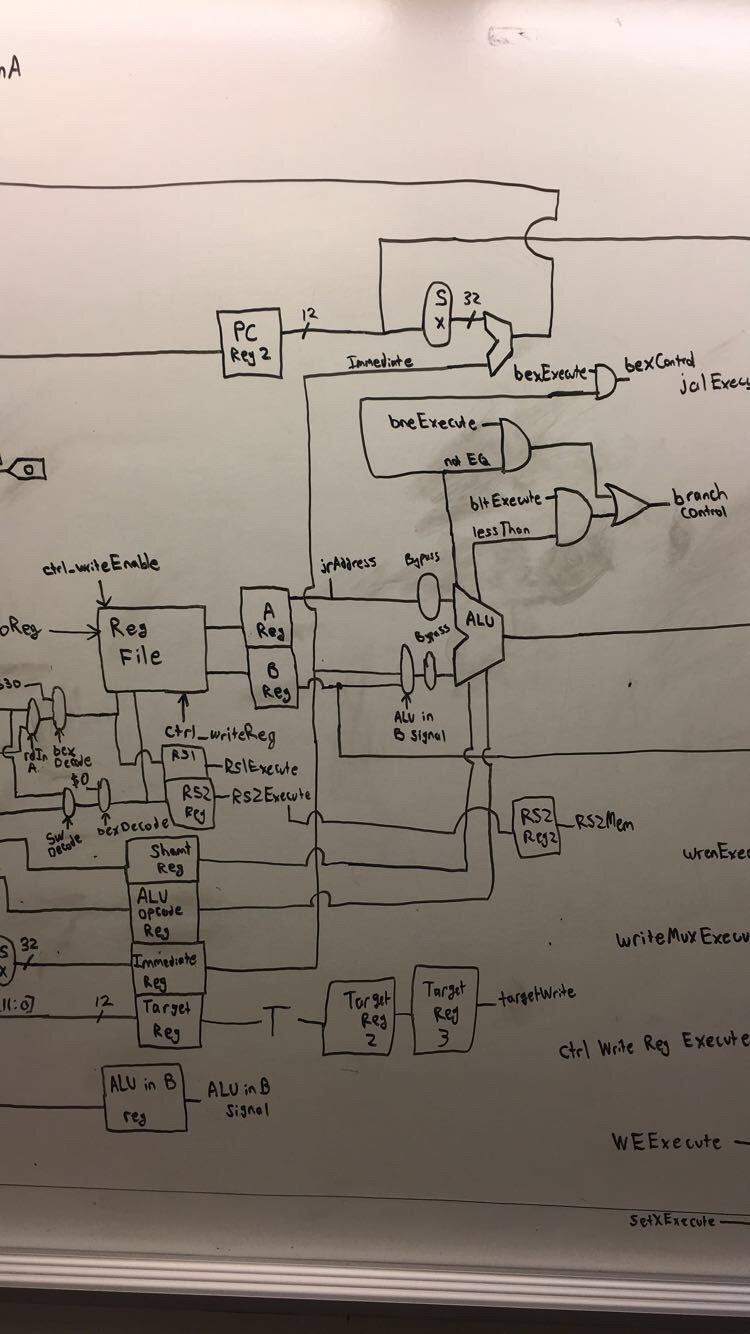
\includegraphics[scale=.45]{Execute.jpg}
        \caption{Execute Stage}
        \label{fig:2}
    \end{figure}
    
       \FloatBarrier
    
\subsection{Memory}

    My Memory stage is similar to the Execute stage in that it also doesn't have much going on because of all the work done in the Decode stage. The output of the ALU is latched and fed into Dmem as the address since the convention of sw and lw are that the address in memory is rs + N; and of course, the control signals for sw and lw made sure that rs was MUXed into ALU input A and the immediate, N, was MUXed into ALU input B. The wren signal which indicates whether or not we write to Dmem is fed into Dmem (the wren signal was decoded in the Decode stage and latched through the Execute stage to get here; the reason I don't immediately feed this control signal into the Dmem when we calculate it in the decode stage is because it corresponds to whether or not we want to write to Dmem for the command that's in a certain stage of the pipeline. If we immediately fed wren into Dmem instead of latching it twice, it would write to Dmem for commands that were two clock cycles prior to the one we actually wanted to write to Dmem. Also, the convention for our ISA is that you load the value of \$rd into Memory[rs + N] so we use our sw control signal to MUX rd into our ctrl\_readB to feed to our RegFile so that the B output of our RegFile corresponds to the data in register rd which can then be latched and fed into the memory stage to be written to Dmem. A picture of my Memory stage is provided below to better elucidate this. \\
        
               \FloatBarrier

  \begin{figure}[!htb]
        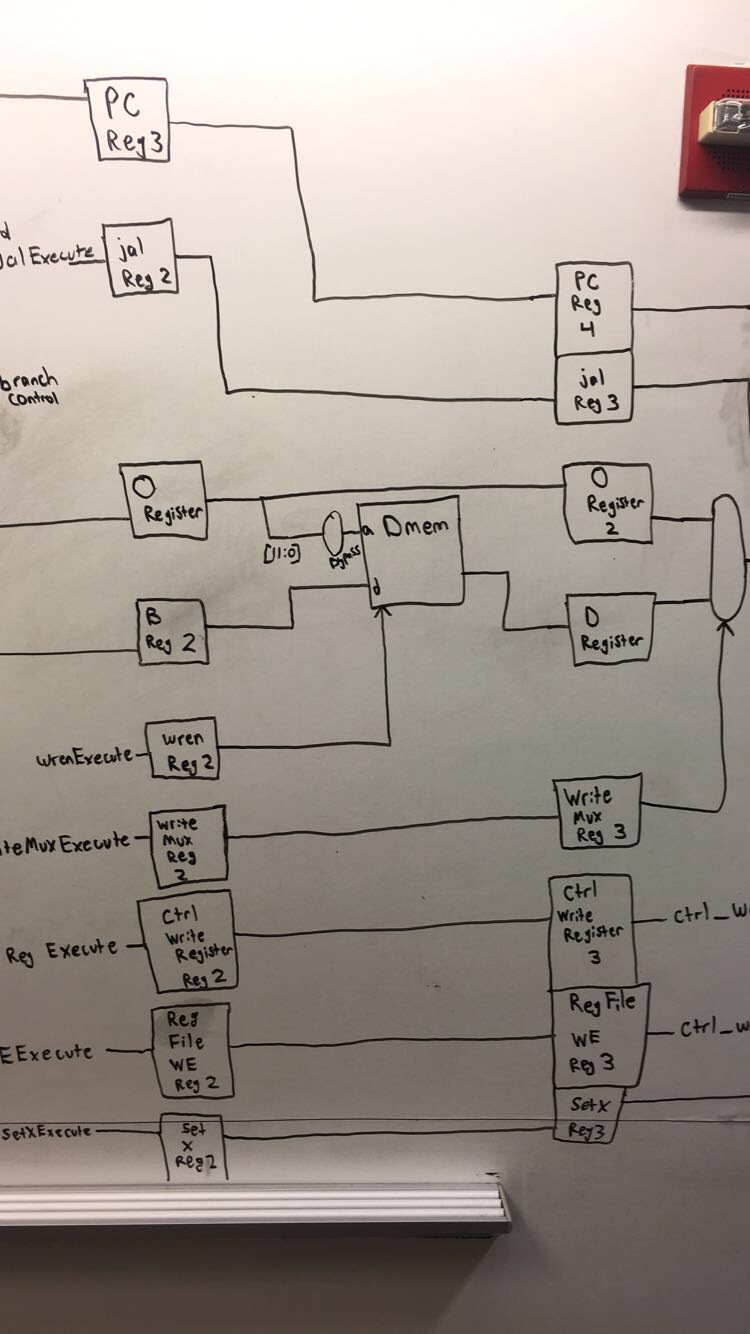
\includegraphics[scale=.45]{Memory.jpg}
        \caption{Execute Stage}
        \label{fig:2}
    \end{figure}
    
       \FloatBarrier

\subsection{Write}

    My Write stage is simply a series of MUXes that decides based on control signals whether or not we write to our RegFile, what we write to our RegFile, and which register we write it to. For example, a jal control signal would be calculated in Decode and latched so that it reached our Write stage 3 clock cycles later so that our Write MUXs know to write the value of PC + 1 to register 31. Or a setx control signal would indicate to the data\_writeReg MUX to choose the T value we extracted during the Decode stage instead of the ALU output (which is usually what we end up writing to our RegFile). A picture of my Write stage is provided below to better elucidate this. Note that not all the MUXs I used are shown below. The ones that aren't there I will discuss in my instructions' implementation details section. \\
    
                   \FloatBarrier

  \begin{figure}[!htb]
        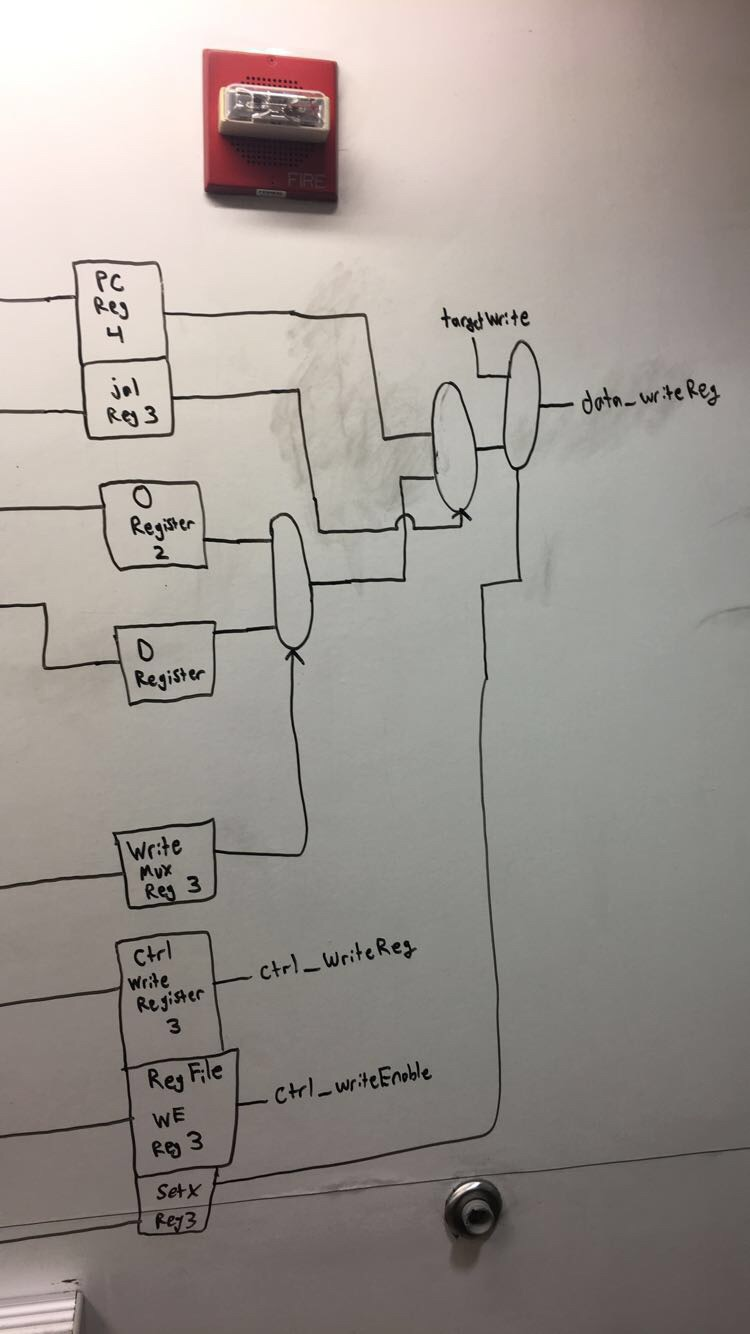
\includegraphics[scale=.45]{Write.jpg}
        \caption{Execute Stage}
        \label{fig:2}
    \end{figure}
    
       \FloatBarrier


\section{Instructions' implementation details}

    \subsection{ALU operations: add, sub, and, or, sll, sra}
        There only command signals required for all of these operations is one indicating that we will write to the RegFile when these operations reach the Write stage. In order to accomplish that, we NOT the instruction's bits [31:27] and then AND them all together (since the opcode indicating ALU operation is 00000). We also have to extract the ALU opcode [6:2] and propagate that to the Execute stage and feed it into the ALU. Although I didn't implement it myself, I realize now that the ALU opcode should be MUXed to avoid doing the wrong operation during commands that aren't ALU based (i.e. if we execute a lw that has bits [6:2] that are supposed to be accounted for as part of its [16:0] immediate, my implementation would mistakenly use those bits as an ALU opcode. If I had more time, I would have MUXed the ALU opcode extracted from Decode with the ALU operation for add (00000) and had the lw, sw, bne, and blt control signals are indications to pick the ALU operation for add instead o the ALU opcode extracted. Since all ALU operations rd = rs operation rt (or rd = rs shifted by shift amount), there is no need to use control signals to MUX in the correct values for rd, rs and rt. \\
    
    \subsection{addi}
        addi requires two MUXs. The first is a MUX that chooses between the immediate and the output of RegFile for B. The second is a MUX that hardcodes to ALU operation to 000000 for add (since the [6:2] bits in an addi command are part of the [16:0] immediate and are not necessarily 000000). We also need to propagate the addi signal forward to indicate that we write to our RegFile when we reach the Write stage. I created a signal called WriteMuxReg that is an OR between the addiDecode Signal and the ALU operation decode signal (since those are the two operations where we pick the output of the ALU to write to the RegFile). I also created a 4-to-1 MUX that chooses between ground, rd, register 31, and register 30 as the register to write to during the Write stage. The reason these are my four choices is because all ALU operations, addi, and lw write to rd, jal writes to register 31, and setx writes to register 30. The 4-to-1 MUX has two control bits. The MSB is an OR between the lw, addi, and ALU operation signals, and the LSB is assigned as the jal control signal. This convention allows the MUX to pick rd when an ALU operation/addi/lw occurs, register 31 when a jal occurs, and register 30 in all other cases (however, the write enable won't be turned on for any other cases besides setx which writes to register 30 anyways). 
        
    
    \subsection{sw}
        The sw signal being a 1 directly means that wren should also be a 1 (which essentially means that we should write to Dmem on a sw). That wren signal is propagated until the Memory stage so that the Dmem knows to write to memory when a sw command reaches it. The sw signal is also part of the OR that feeds into the ALU in B signal (that when high chooses the immediate over the RegFile B output). This is because the convention of sw is that Mem[rs + N] = rd. rs is by default the A input to the ALU so there's no need to change that. sw also requires the ALU addition opcode to be forcibly fed into the ALU. This is achieved in the same way as the addi command, an OR gate whose input is the sw, lw, and addi signal being propagated forward from when it was calculated in the Decode stage.
    
    \subsection{lw}
        Similar to a sw command, the lw command requires that the ALU in B be the immediate which is why the lw signal is one of the inputs to the ALU in B OR gate. lw also means that the register we will write to during the Write stage will be rd which is why the MSB for the MUX that chooses ctrl\_writeReg is the output of an OR gate whose inputs are the addi, ALU operation, and lw signals. Also, the command signal that propagates to the RegFile's write enable during the Write stage is the output of an OR gate for which the lw signal is one of the inputs (because we do need ctrl\_writeEnable to be a 1 when the lw commands gets to the Write stage of the pipeline). The lw also uses the same MUX that the sw and addi command used to force the ALU to perform additions regardless of the bits in [6:2] of the current command. 
        
        
    \subsection{j}
        The jump command is different than all the previous operations implemented in that it does not require any arithmetic. Albeit, the ALU still produces an output when a j command comes to the Execute stage, but that output is nonsense and should be ignored. In order to implement j, the j control signal has to be propagated to Execute where it is fed into one of the previously mentioned PC MUXes that chooses the T value of the corresponding J command as the new input to the PC. Nothing else is required from a J command so we keep wren at 0 and ctrl\_writeEnable at 0 to avoid overwriting our data with nonsense. When the J control signal is fed into the PC MUX in its execute stage, it also triggers the NoOp signal (the NoOp signal is an OR between the J control signal and various other control signals that require flushing the pipeline). The NoOp signal makes it so that the q\_imem (the current instruction being fetched) that's fed into the Instruction latch right before the Decode stage is all 0's and all the control signals fed from the Execute stage to the Memory stage are all 0's. This essentially "flushes" the previous two commands out of the pipeline since we don't want anything after the jump command to actually occur (or else we'd call it the wait2CyclesAndtThenJump command). The reason an all 0's command flushes the pipeline is because it is essentially tricking the processor into thinking the command it needs to execute is add register 0 (which is hardcoded to 0) to register 0 and then put it inside register 0 (which can't even be written to based on my RegFile implementation choices).
    
    \subsection{bne}
        The way I implemented not equal in my ALU is XORing (with a custom build XOR module, not the build in Quartus one) all the bits of A and B together, and ANDing their inverses. The reason for this is because the XOR of two bits that are the same is always 0; the not of 0 is always 1; and the AND of all 1's is always 1. This logic yields a control signal that is only high when the ALU inputs A and B are not equal. This ALU control signal is then ANDed with the bne control signal (that was propagated to Execute from Decode) to decide whether or not both conditions required for a bne (that A != B and a bne command is currently occurring) are satisfied. bne also requires the previously mentioned rdInA MUX since bne compares rd to rs. bne requires another MUX on top of that which chooses rs to be the B input to the ALU (since rt is the default B input). The NoOp signal also has to be set to high. This is why one of the inputs to the NoOp signal OR gate is a control indicating whether or the bne conditions where met. My convention is using delayed branching so there are two NoOp MUXes and the branch has a two cycle delay.
    
    \subsection{jal}
        jal was a fairly straightforward command to implement. The only control signals you require are one to tell the Write stage to write the PC+1 value (which is latched in the PC latches that are present in each stage) to register 31. This is accomplished using two MUXs: one chooses between the output of some previous MUX and 11111 (for register 31) for ctrl\_writeReg and the other chooses between the output of some other previous MUX and PC + 1. 
        The NoOp signal should also be set to high when a jal is called which is why one of the inputs to the NoOp signal OR gate is a control indicating that a jal is occurring. 
        
    \subsection{jr}
        jr was also a fairly straightforward command to implement. The only control signals jr requires is one that tells a MUX in the Fetch stage to choose the value in rd as the new PC instead of PC + 1 (which is what it would pick by default) and one that tells the RegFile to grab the register described by rd as its A output. The first control signal effects a MUX in the Fetch stage but it isn't actually set to high until the Execute stage. This is to avoid changing the PC too early. The second control signal is the input (not the select bits) to the MUX. The reason for this is because the jr signal tells the RegFile to grab the value in rd and place it in the A input of the ALU and then the jr control signal also tells the one of the PC MUXs to set the PC input to the A input of the ALU instead of PC + 1. jr also requires us to flush the pipeline which is why, just like jal, bne, and j, the jr control signal is an input to the OR gate that outputs the NoOp signal. 
        
    
    \subsection{blt}
        The blt command requires the ALU to perform subtraction. The way I implemented less than in my ALU is by subtracting B from A and checking if the result is negative or positive (by extracting the MSB which would be a 1 for a negative number and a 0 for a positive number). This logic yields a control signal that is 1 when A < B which is the condition for blt to branch. This control signal is ANDed with the blt control signal so that we know when both the conditions for a blt are met. If this control signal is high, the pipeline is flushed with NoOps (just like in jr, jal, bne, and j) and one of the PC MUXs chooses the output of the adder that adds the immediate with PC + 1. blt requires the same MUXed inputs to the ALU as bne. Therefore the control signals that put rd into ALU input A and rs into ALU input B are an OR between the blt control signal and the bne control signal. My convention is using delayed branching so there are two NoOp MUXes and the branch has a two cycle delay.
    
    \subsection{bex}
        bex is different from other branch commands in that it sets the PC to T. This small difference in implementation simply requires another MUX that chooses between the default PC + 1 and T depending on the bex control signal. The bex control signal is also fed into two MUXs make it so that the A input to the ALU is the value in register 30 (which is \$rstatus) and the B input to the ALU is the value in register 0 (which is hardcoded as 0). We do this because then the not equal signal from the ALU will be high when \$rstatus != 0 which is the condition for bex to branch. This is not equal output is then ANDed with bex control signal to make sure that the two conditions for bex are met (that a bex is actually occurring and that \$rstatus is actually != 0). My convention is using delayed branching so there are two NoOp MUXes and the branch has a two cycle delay.
    
    \subsection{setx}
        setx doesn't require the use of any control signals until you reach the Write stage. You essentially propagate T and the setx control signal to the Write stage and feed those into the input of MUXs that choose between what would have been the value of ctrl\_writeReg and data\_writeReg if a setx wasn't occurring and register 30 (or \$rstatus) and whatever T is respectively. We also have to make sure that the ctrl\_writeEnable is 1 so we have to set one of the inputs to the OR gate that outputs that control signal that gets propagated to ctrl\_writeEnable to the control signal for setx. 

    \subsection{Bypassing}
        In order to implement bypassing, I saved the rs1 and rs2 value from the Decode stage in a latch so that we can use them in the Execute stage. In the Execute stage, I use the ctrl\_writeReg signal to compare if what is going to be written into the RegFile soon is an argument of a command 2 or less stages after (i.e. if command A is in Decode, you grab rd from command B if it is in Memory or Execute). The logic for this is fairly simply. I used a 5-bit comparator that uses custom made XORs. The 5-bit comparator is hardcoded such that if any of the inputs are 0, the output is automatically 0 (this is to avoid an infinite bypass loop for when NoOps are occurring). If the inputs are not 0, then the XORs XOR all the individual bits from input A and input B and if the AND of the inverse of those XOR outputs is 1, then they are equal (this is because the XOR of two bits that are the same is always 0, the inverse of 0 is always 1, and the and of all 1's is 1). The logic I just mentioned is the bypass logic for my Decode Bypassing. The logic for my Memory Bypassing is different. The Memory bypass only occurs if you are about to write something a register and the command after that is saving that register value to memory. In this situation, you take the output that you were about to write to register X and put that into the argument for the sw command that will write the new value of register X into Dmem. The logic for checking if rd in Write is the same as the argument in Memory is very similar. It involves a 5-bit comparator again that uses XOR's in the same way as the previous bypass logic. The only difference is that you only have to check B's register because B is the only thing that can be written to Dmem. 
        
                       \FloatBarrier

  \begin{figure}[!htb]
        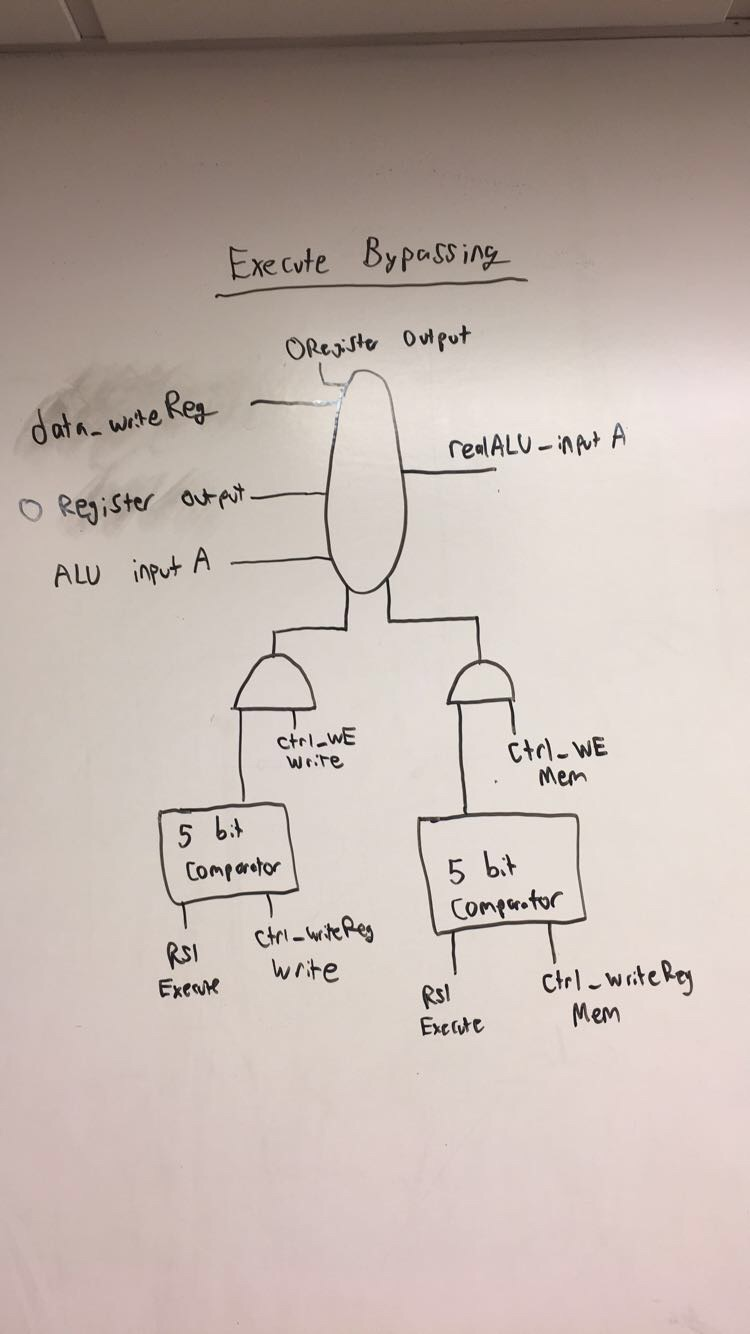
\includegraphics[scale=.45]{ExecuteBypassing.jpg}
        \caption{X/W Bypassing}
        \label{fig:2}
    \end{figure}
    
      \FloatBarrier

  \begin{figure}[!htb]
        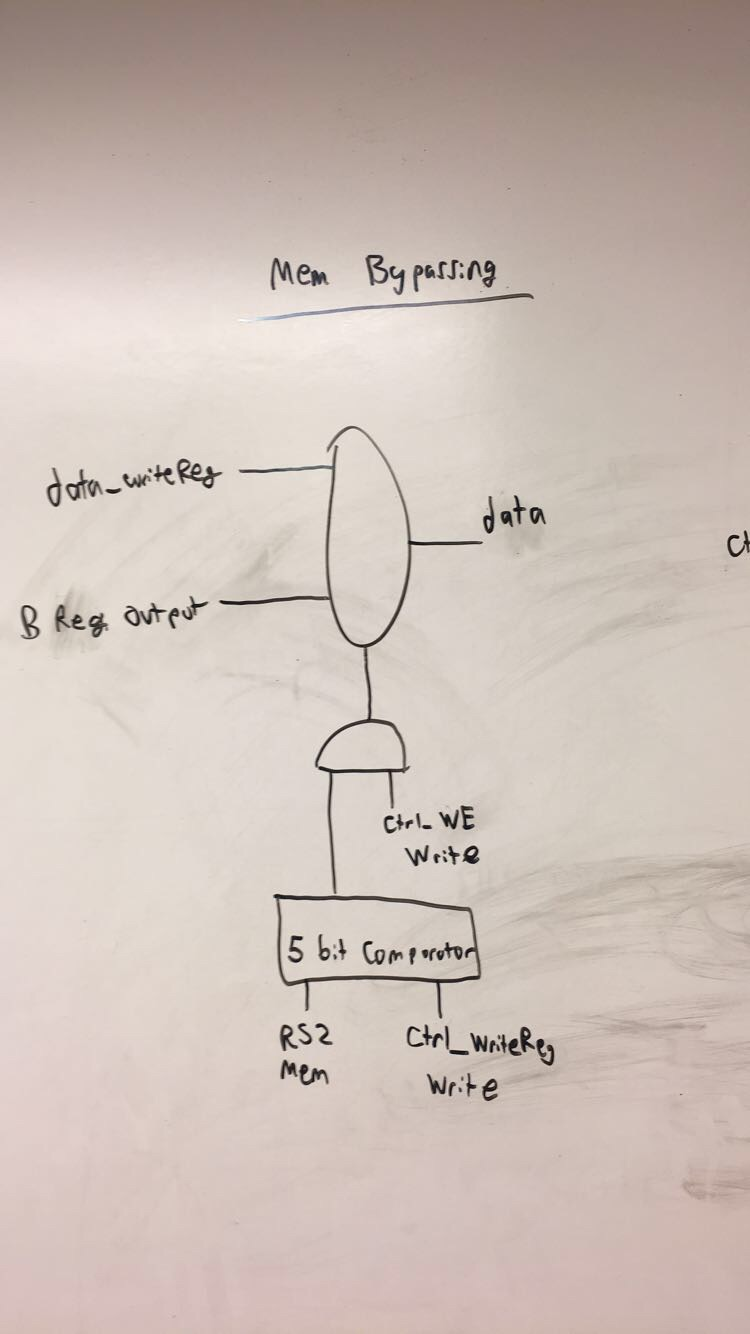
\includegraphics[scale=.45]{MemBypassing.jpg}
        \caption{M/W Bypassing}
        \label{fig:2}
    \end{figure}
    
       \FloatBarrier
    
    \subsection{Flushing}
        In order to implement flushing, I created a control called a NoOp signal. That NoOp signal is the output of an OR gate that takes in all the control signals associated with commands that require flushing (i.e. jr, jal, bne, blt, bex). In order to properly flush my pipeline, I have a NoOp MUX that feeds into the F/D latch and a NoOp MUX that feeds into the control signals that are given to the Memory stage. The reason the NoOp MUXs are at the end of each stage instead of the beginning is because that would cause a combinational logic loop that would lead to undefined behavior since the inputs to the signals that trigged the NoOp signal would change when the NoOp signal is triggered. This effectively flushes the pipeline and in an efficient manner because it prevents the instructions behind whatever instruction triggered to flush from propagating forward. Since instructions that cause flushes are resolved in the Memory stage, the Fetch stage and the Execute stage are the only ones with the NoOp MUX. 
    
    \subsection{Stalling}
        The only situation in which you need stalling is if you load something into a register and then immediately try to access that new value. The reason you can't bypass is because loading occurs on the falling edge of the clock meanwhile bypassing would occur on the positive edge of the clock. This would lead to us bypassing with the wrong value. The logic behind stalling is simply an AND between the inverse of whether or not there is a sw in the Fetch stage, a lw in the Decode stage, and if rs1 for the operation in the Fetch stage == rd for the load that is currently in the Decode stage or if rs2 for the operation in the Fetch stage == rd for the load that is currently in the Decode stage. Stalling behavior is implemented by MUXing the next default address of the PC (PC + 1) with the current value of the PC. This essentially keeps the PC constant until the stall control is no longer 1. 

\pagebreak

\section{Testing instructions and challenges}

\subsection{ALU, sw, lw, j \& bypass test}
\begin{verbatim} 
addi $1, $0, 5
sw $1, 8(0)
nop
nop
lw $2, 8(0)
add $3, $1, $2 
addi $4, $1, 23
and $5, $4, $1
or $6, $4, $1
sll $0, $5, 2
sra $16, $6, 4 
sub $17, $0, $16
j 1
addi $1, $0, 1

\end{verbatim}

   \FloatBarrier

  \begin{figure}[!htb]
        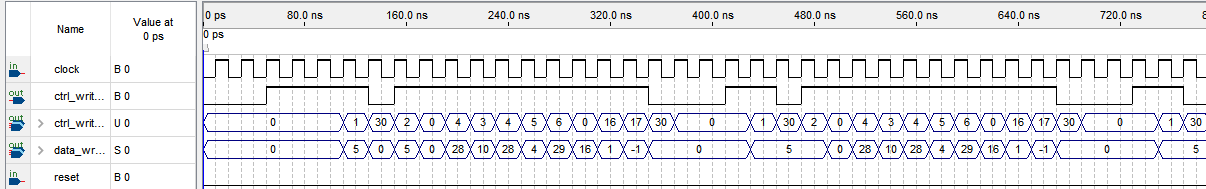
\includegraphics[scale=.5]{ALUtest.PNG}
        \caption{ALU, j, bypass, sw, lw Test}
        \label{fig:2}
    \end{figure}
    
       \FloatBarrier
       
\pagebreak

\subsection{jal & jr}
\begin{verbatim}
addi $1, $0, 1
jal 3
add $1, $1, $1
jr $31
addi $1, $0, 2

\end{verbatim}

   \FloatBarrier

  \begin{figure}[!htb]
        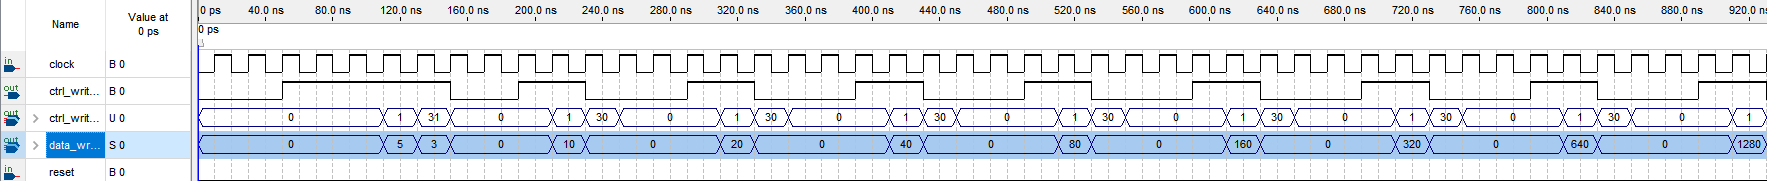
\includegraphics[scale=.4]{jaljrTest.PNG}
        \caption{jal \& jr Test}
        \label{fig:2}
    \end{figure}
    
       \FloatBarrier

    
\subsection{bne (taking branch)}
\begin{verbatim}
addi $1, $0, 1
addi $2, $0, 2
bne $1, $2, 2
addi $1, $0, 2
addi $2, $0, 4
sub $4, $1, $2  

\end{verbatim}

   \FloatBarrier

  \begin{figure}[!htb]
        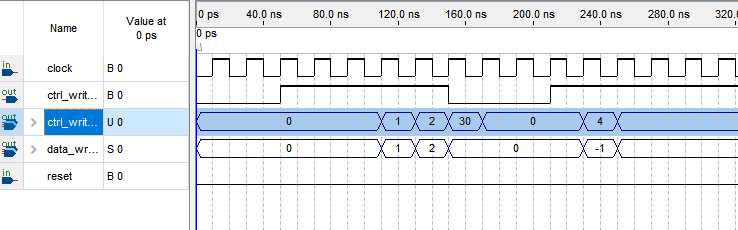
\includegraphics[scale=.8]{bneTest.PNG}
        \caption{bne Test}
        \label{fig:2}
    \end{figure}
    
    \FloatBarrier

\pagebreak

    
\subsection{bne (not taking branch)}
\begin{verbatim}
addi $1, $0, 3
addi $2, $0, 3
bne $1, $2, 2
addi $1, $0, 2
addi $2, $0, 4
sub $4, $1, $2 

\end{verbatim}

   \FloatBarrier

  \begin{figure}[!htb]
        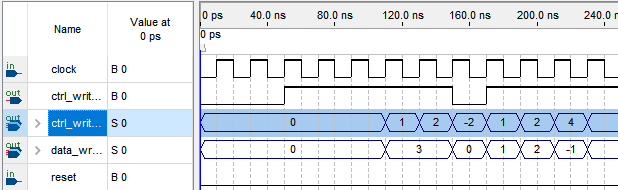
\includegraphics[scale=.9]{bneTest2.PNG}
        \caption{bne Test 2}
        \label{fig:2}
    \end{figure}
    
       \FloatBarrier
    \pagebreak
    
\subsection{blt (taking branch)}
\begin{verbatim}
addi $1, $0, 1
addi $2, $0, 2
blt $1, $2, 2
addi $2, $0, 4
addi $1, $0, 2
sub $4, $1, $2

\end{verbatim}

   \FloatBarrier
      \begin{figure}[!htb]
        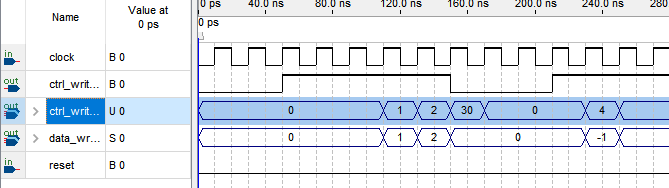
\includegraphics[scale=.9]{bltTest.PNG}
        \caption{blt Test}
        \label{fig:2}
    \end{figure}
    
       \FloatBarrier
    
    
\subsection{blt (not taking branch)}
\begin{verbatim}
addi $1, $0, 3
addi $2, $0, 2
blt $1, $2, 2
addi $2, $0, 1
addi $1, $0, 2
sub $4, $1, $2 

\end{verbatim}
   \FloatBarrier
  \begin{figure}[!htb]
        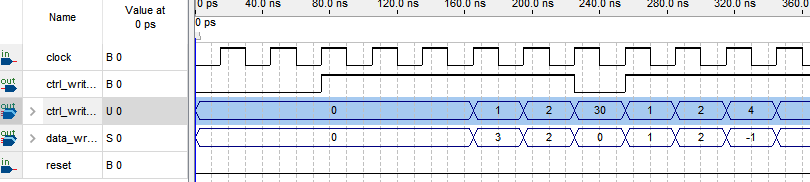
\includegraphics[scale=.7]{bltTest2.PNG}
        \caption{blt Test 2}
        \label{fig:2}
    \end{figure}
       \FloatBarrier
    
    
\subsection{bex (not taking test)}
\begin{verbatim}
bex 64
addi $1, $0, 1

\end{verbatim}
   \FloatBarrier
  \begin{figure}[!htb]
        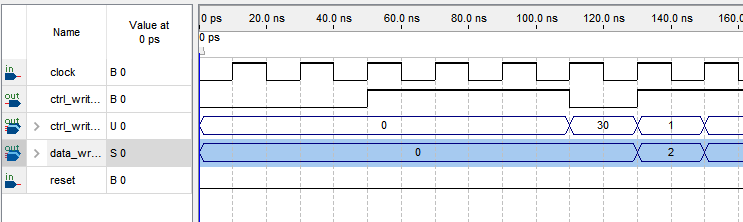
\includegraphics[scale=.5]{bexTest.PNG}
        \caption{bex Test (note that 1 is written into \$rstatus to indicate add overflow}
        \label{fig:2}
    \end{figure}
       \FloatBarrier
    
    
\subsection{bex (taking branch)}
\begin{verbatim}
addi $1, $0, 1
sll $2, $1, 11110
add $1, $1, $1
nop
nop
bex 16
addi $1, $0 1

\end{verbatim}
   \FloatBarrier
  \begin{figure}[!htb]
        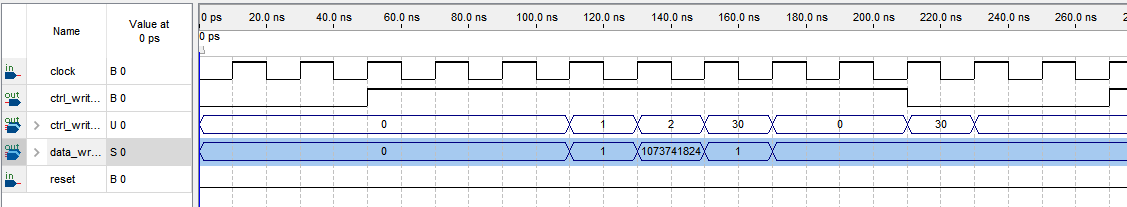
\includegraphics[scale=.5]{bexTest2.PNG}
        \caption{bex Test (note that 1 is written into \$rstatus to indicate add overflow}
        \label{fig:2}
    \end{figure}
       \FloatBarrier
    
    
    \pagebreak
\subsection{setx}
\begin{verbatim}
addi $1, $0, 1
addi $1, $0, 1
sll $2, $1, 11110
add $1, $1, $1
nop
nop
setx 0
nop
nop
bex 64
addi $4, $30, 0

\end{verbatim}

  \begin{figure}[!htb]
        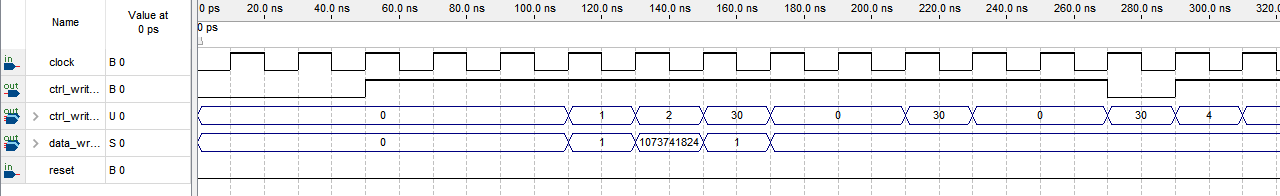
\includegraphics[scale=.45]{setxTest.PNG}
        \caption{setx Test}
        \label{fig:2}
    \end{figure}
    


\section{Known issues with processor}

    \subsection{Hold time violation}
        For some reason, timed simulations give me hold time violations. When I open the tab to check timing requirements, it says that I have unnecessary levels of combinational logic. I'm not exactly sure what this means. What's really confusing me is that it says that the hold time violation is being caused by these "23 extra levels of logic" that I have, but that doesn't seem to make sense because there is no hierarchical logic that is 23 stages long in any part of my pipeline. I thought that the hold time violation may be due to the fact that I have some latch outputs that connect directly to other latch inputs and, during the rising clock edge, the value may not be steady for long enough. But I'm not at all sure why my timing is off. This leads to a lot of issues. Sometimes my bypass values are wrong/the right value is calculated in time to be written to a register. However, as shown by the waveforms above, my processor seems to be almost fully functional when running simulations without timing.
        
    \subsection{Bypassing}
        Refer to the waveform for my ALU, j, lw, sw, and hazards test. For some reason register 4 is having 28 written to it before it is supposed to. I believe that this is because there might be a small runtime error with my bypass logic somewhere. Register 4 is still correctly written at the end of the instruction execution, but the fact that it's being written two clock cycles early is something I think has to be because of a faulty bypassing implementation.
    
    \subsection{ALU not equal and less than}
        I never actually got to check my new ALU not equal and less than implementations using the TA test bench, so I'm not sure if they work. I'm pretty sure they do. But I was also pretty sure the last time and clearly I was wrong.
        
    \subsection{Mult/Div}
        MultDiv doesn't work because I didn't have time to implement it. If a Mult/Div command is entered, the processor will recognize the opcode as an ALU operation, but since the ALU opcode isn't something it recognizes, it'll default to addition. Both Mult/Div just result in addition. 
        
\section{Challenges \& What I learned}

    The biggest challenges I faced in creating this processor were mostly with timing. A lot of the times things that I thought would be located in a certain part of the processor were not actually there when I thought they were, so I ended up extracting the wrong values when trying to obtain the value in question. I now definitely have a stronger appreciation for the importance of timing and delays in circuits. In the past, I've really only dealt with idealized digital circuits. Having to worry about efficiency and gate delays definitely adds a whole different dimension to digital circuit analysis. It forces you to be very conscious of how many levels of combinational logic you're using and how many inputs you have to those gates and how much hardware you're wasting. I definitely have an appreciation for the balance between using more/less hardware and using more/less levels of combinational logic to try and achieve maximum efficiency. \\
    
    Another challenge I faced was regarding Verilog syntax. There were often times when I treated it too much like a sequential HLL instead of a HDL with concurrent operation. This led to many combinational logic loops that I had to spend hours debugging. What I learned from this was that it's definitely in my best interest in the future to draw the circuit as I go. As soon as I started drawing my circuits out while parsing through my code line by line, I very quickly found all the issues with my code. It was much more apparent to me when I could actually see how all the wires connected.
    
    

    
\end{document}
